\section*{К155ИЕ6}
\addcontentsline{toc}{section}{К155ИЕ6}

\subsection*{Построение деманстрационной модели К155ИЕ6}
\addcontentsline{toc}{subsection}{Построение деманстрационной модели К155ИЕ6}

В данной части построим синхронный счетчик К155ИЕ6. Данный счетчик имеет несколько входов:

\begin{itemize}
    \item A-B \textbf{---} информационный численны вход
    \item $\sim$LOAD$\sim$ \textbf{---} при установленной логической 1 загружает значение из информационного входа
    \item CLR \textbf{---} сбрасывает текущее значение счетчика при установленной логической единице
    \item UP и DOWN \textbf{---} производит счет $+1$ и $-1$ соответсвтенно. Счет происходит по положительному перепаду входного сигнала ($0 \rightarrow 1$) 
\end{itemize}

\begin{figure*}[h!]
    \centering
    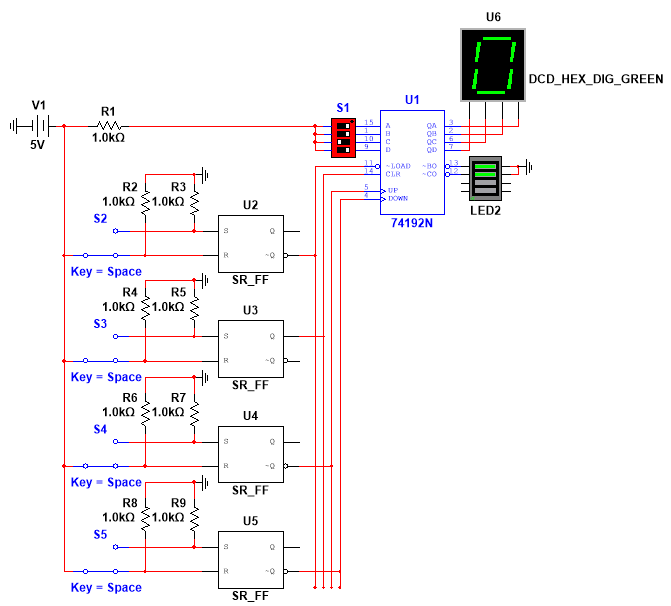
\includegraphics[scale=0.8]{images/image-8.png}
    \captionof{figure}{Счетчик К155ИЕ6}
    \label{image:8}
\end{figure*}

Выше представлена деманстрационная модель с счетчиком К155ИЕ6. Протестируем работы счетчика на данной модели. \par

\newpage 

\textbf{Загрузка значения в счетчик.} Для загрузки значения выставим переключатели информационных входов,
например, в значение 9. Затем на вход LOAD подадим логическую 1.

\begin{figure*}[h!]
    \centering
    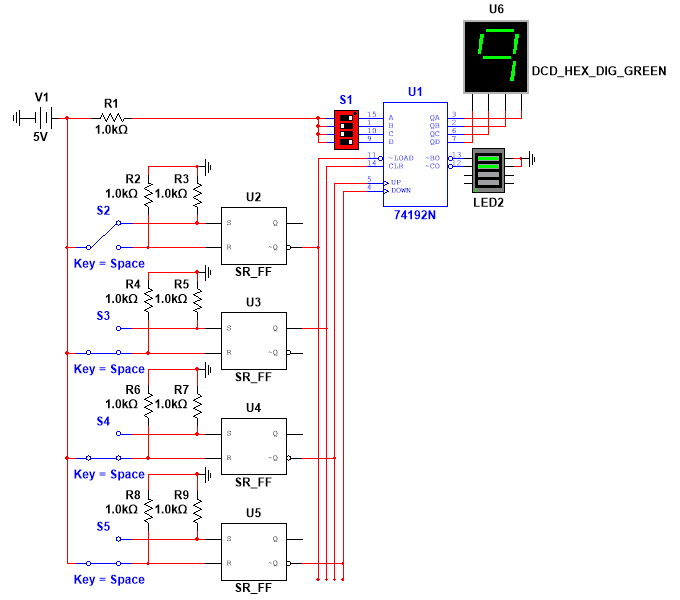
\includegraphics[scale=0.8]{images/image-9.png}
    \captionof{figure}{Загрузка значения 9 в счетчик}
    \label{image:9}
\end{figure*}

На дисплее видим значение $9_{16}$. Результата соответвует ожиданию. \\[1mm]

\newpage

\textbf{Сброс установленного значения.} Для сброса значения необходимо подать логичкую 1 на вход CLR.
Сбросим ранее загруженную 9, ожидаем на дисплее значение $0_{16}$.\par

\begin{figure*}[h!]
    \centering
    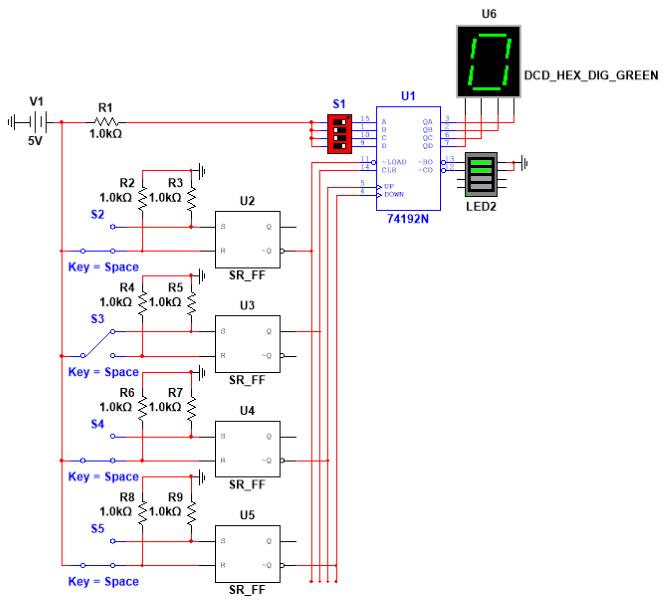
\includegraphics[scale=0.8]{images/image-10.png}
    \captionof{figure}{Сброс значения счетчика}
    \label{image:10}
\end{figure*}

Видим на дисплее значение $0_{16}$. Результат соответвует ожиданию. К слову, вход сброса значения имеет приоритет над входом загрузки - 
нельзя загрузить значение, если на вход сброса подана 1. \par

\textbf{Инкремент и дикремент значения.} Загрузим в счетчик значение 5, на вход UP последовательно будем подавать перепад $0 \rightarrow 1$.
Ожидаем увеличение значения на 1 при каждой интерации. Значение ожидаемо увеличивается на 1. Аналогично был проверен дикремент.

\newpage

\subsection*{Исследование счетчика при суммирование в динамике}
\addcontentsline{toc}{subsection}{Исследование счетчика при суммирование в динамике}

Подключим вход UP к переодичному источнику сигнала. Выходы подключим к логическому анализатору. Выставив 
частоту источника пронаблюдаем изменения значения на дисплее и в логическом анализаторе. Видоизменная схема
счетчика представленна ниже. \par

\begin{figure*}[h!]
    \centering
    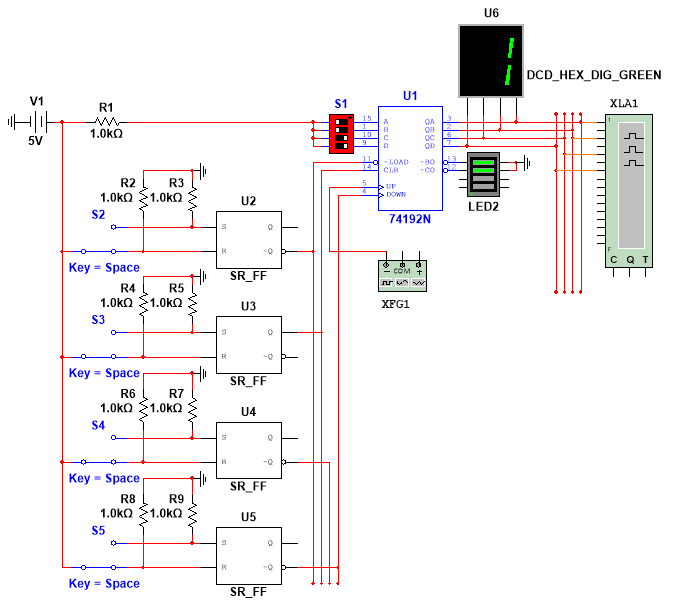
\includegraphics[scale=0.7]{images/image-11.png}
    \captionof{figure}{Счетчик с анализатором}
    \label{image:11}
\end{figure*}

В анализаторе видно порядок изменения сигналов на выходе. Изменения соответвуют изменниям значения на дисплее.

\begin{figure*}[h!]
    \centering
    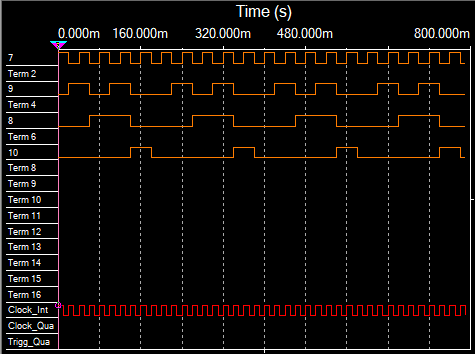
\includegraphics[scale=0.6]{images/image-12.png}
    \captionof{figure}{Анализатор}
    \label{image:12}
\end{figure*}